
\subsection{Phân tích tài nguyên sử dụng}

Dựa trên kết quả từ bảng báo cáo, hệ thống sử dụng một lượng tài nguyên rất nhỏ so với tổng thể chip FPGA mục tiêu.

\begin{figure}[H]
    \centering
    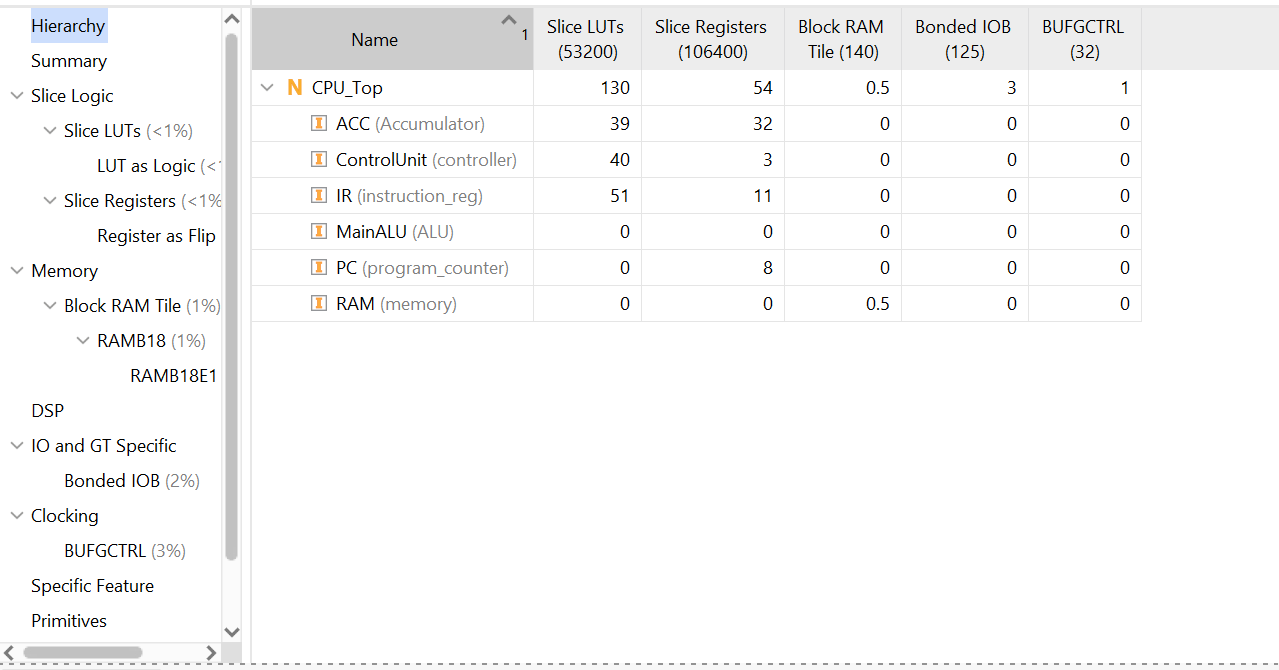
\includegraphics[width=0.9\textwidth]{ulti.png}
    \caption{Báo cáo tài nguyên Utilization chi tiết cho từng module}
    \label{fig:utilization}
\end{figure}


\subsection{Phân tích thời gian }

\begin{figure}[H]
    \centering
    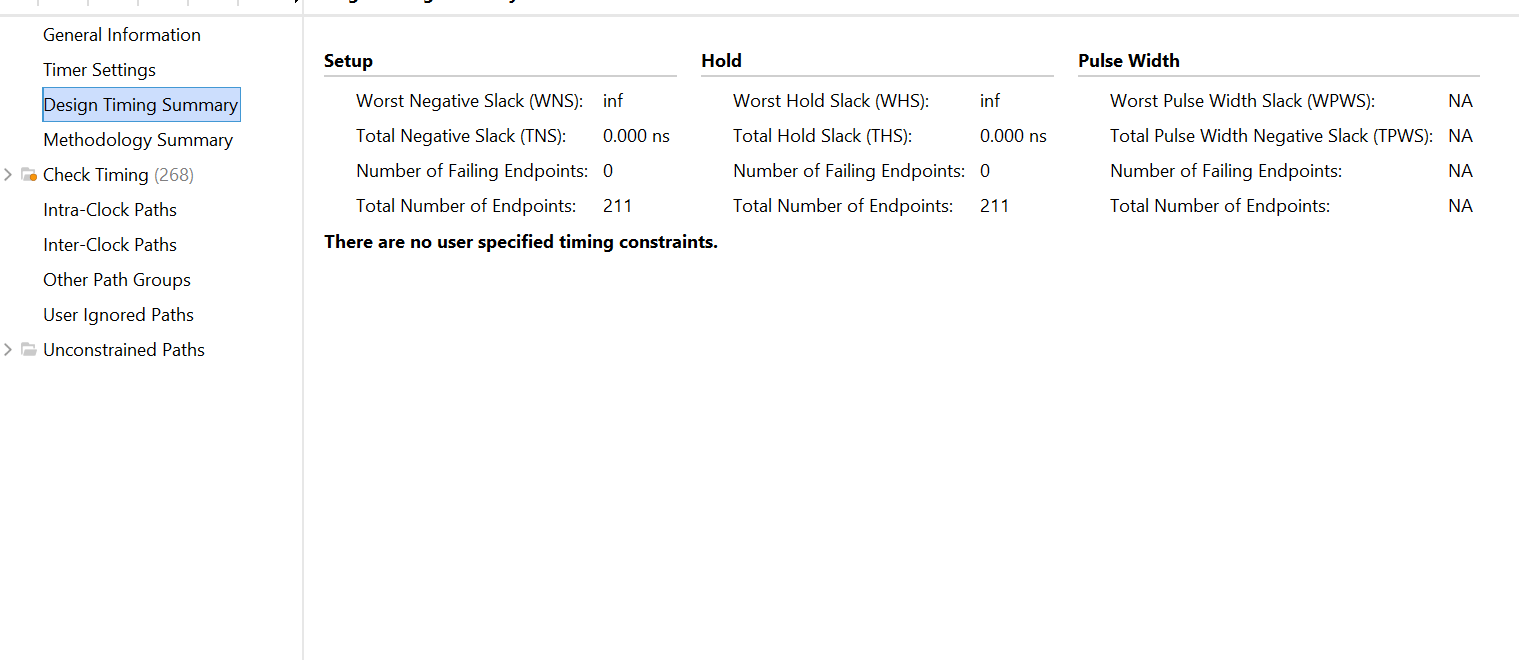
\includegraphics[width=0.9\textwidth]{time.png}
    \caption{Báo cáo phân tích thời gian Timing Summary}
    \label{fig:timing}
\end{figure}

\textbf{Nhận xét:}
\begin{itemize}
    \item \textbf{Độ tin cậy:} Chỉ số TNS (Total Negative Slack) bằng 0.000 ns và không có điểm lỗi cho thấy thiết kế ổn định.
    \item \textbf{Khả năng vận hành:} Mặc dù chưa thiết lập ràng buộc XDC cụ thể cho xung clock,
     nhưng với mật độ logic thấp hệ thống có thể đáp ứng tốt các ứng dụng yêu cầu tần số hoạt động 100MHz.
\end{itemize}

\subsection{Phân tích năng lượng tiêu thụ}

\begin{figure}[H]
    \centering
    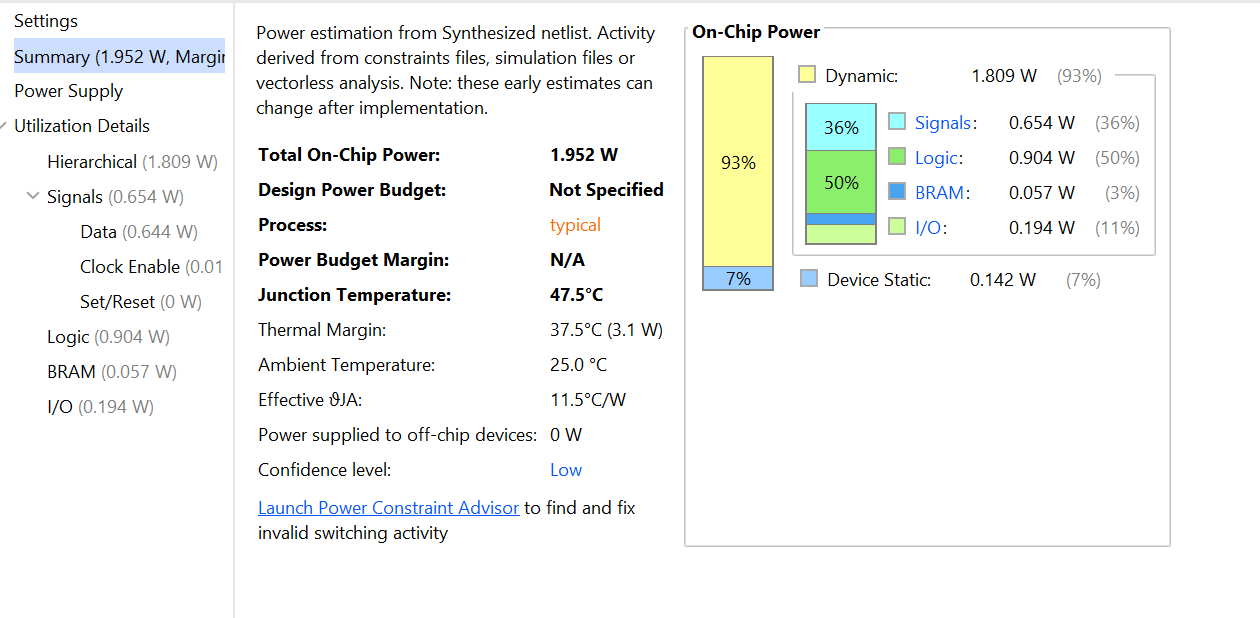
\includegraphics[width=0.8\textwidth]{power.png}
    \caption{Báo cáo ước tính năng lượng tiêu thụ và nhiệt độ hoạt động}
    \label{fig:power}
\end{figure}

\textbf{Nhận xét:}
\begin{itemize}
    \item \textbf{Hiệu suất năng lượng:} Tổng công suất tiêu thụ đạt 1.952 W. Trong đó, công suất động (Dynamic Power) chiếm tới 93\%, 
    cho thấy phần lớn năng lượng được tập trung cho các hoạt động đóng cắt cổng logic để xử lý lệnh.
    \item \textbf{Phân tích thành phần:} Logic chiếm 50\% và tín hiệu chiếm 36\% công suất động.
    \item \textbf{Độ ổn định nhiệt:} Nhiệt độ hoạt động duy trì ở mức 47.5°C. Đây là mức nhiệt lý tưởng để CPU có thể vận hành liên tục mà không bị quá nhiệt.
\end{itemize}